\chapter{Meilleur connecteur}

Regardons l'algorithme donné \ref{sec:revueAlgorithme} d'un point du vue
graphe.
Au premier indice (\ref{eq:al1}), on répond par le terme le plus activé, c'est
à dire le voisin le plus activé.
A partir du second indice (\ref{eq:al2}), l'intersection des deux termes est
faite, et le terme le plus activé est proposé. Cela revient à obtenir les
voisins directs communs aux termes, et proposer le plus activé.

On suivra ici la même logique, mais plutôt que de rechercher les voisins
communs à distance 1, on cherchera les voisins communs à distance $L$ avant
de proposer le meilleur.

%\medskip
% Plan
% On va d'abord voir comment trouver l'ensembles des meilleurs connecteurs
% Puis, comment leur donner un order, pour déterminer LE meilleur connecteur

\section{Calcul des chemins}

Étant donné un ensemble d'indices $I \subseteq V$ de $k > 1$, on cherche à
trouver l'ensemble des meilleurs connecteurs, noté $C_{I} \subseteq \bar{I}$,
c'est à dire les sommets connectant le plus de paires d'indices.
On appelle connecteur un sommet se trouvant sur au moins au chemin
élémentaire reliant une paire d'indice.
Plus le chemin est long, moins il est pertinent, on décide donc de limiter la
longueur\footnote{On pourrait aussi fixer à un poids moyen (comme
approximation de la pertinence) minimum.} à $L$.

\medskip

Plus formellement, on se donne la fonction $M_{L}$ qui, à une paire de sommets
distincts, associe l'ensemble des chemins de longueur maximum $L$
les connectant.
On veut trouver les $c$ :
\begin{align*}
	C_{I} = \{ c \in \bar{I} \text{ tel que } | \, \{ (i, i') \, : \, (i, i') \in \mathcal{P}_{2}(I) \, / \, \exists \mu \in M_{L}(i, i') \, \text{avec } c \text{ une extrémité dans } \mu  \} \, |_{MAX}\}
\end{align*}

Prenons par exemple le graphe de la figure \ref{fig:exemple1}.
Les rectangles sont des indices ($I = \{ A, B, C \}$) et les cercles des
sommets quelconques.
La direction des relations n'ayant pas d'importance, le graphe est non-orienté.
Ici, avec $L = 3$, on a $C_{I} = \{1, 2, 3 \}$ car ils connectent toutes les paires :
A--B, A--C, B--C. Les sommets $4$ et $5$ ne connectent pas B--C et A--B
respectivement.

\begin{figure}[H!]
	\centering
	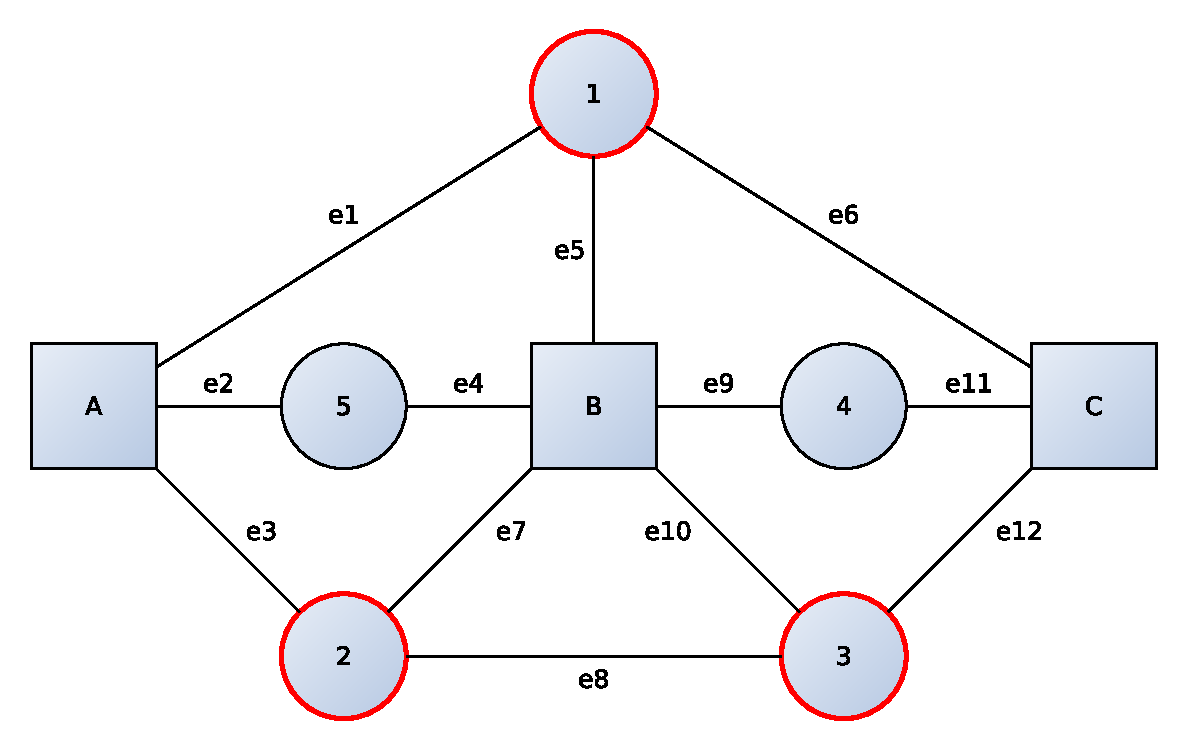
\includegraphics[scale=0.60]{./img/exemple1}
	\caption{Exemple $C_{I}$}
	\label{fig:exemple1}
\end{figure}

Le calcul des chemins pour une paire d'indices $(i, i')$ est possible à l'aide
d'un parcours en profondeur.
\begin{todo}
	Expliquer algorithme
\end{todo}
\begin{todo}
	Complexité : $O(k.m)$.
\end{todo}

%\begin{algorithm}
%	\SetKwFunction{CalculerChemins}{calculerChemins}
%	\SetKwFunction{Visiter}{visiter}
%	\SetKwData{Src}{src}
%	
%	\Entree{$G = (V, E), \: I \subseteq V, \: L \in \mathbb{N}^{+}$}
%	\Res{Construit $M_{L}$}
%	
%	\Deb{
%		$M_{L} \leftarrow \{\}$ \\
%		\PourCh{$\Src \in I$}{
%			$D \leftarrow I \setminus \{ \Src \}$ \\
%			$\Visiter(\Src)$
%		}
%	}
%	\caption{calculerChemins}
%	\label{alg:calculerChemins}
%\end{algorithm}
%
%\begin{algorithm}
%	\SetKwFunction{Marque}{marque}
%	\SetKwFunction{Visiter}{visiter}
%	\SetKwFunction{Dernier}{dernier}
%	\SetKwFunction{Voisins}{voisins}
%	\SetKwFunction{SupprDernier}{supprDernier}
%	\SetKwData{CheminCourant}{$\mu$}
%	\SetKwData{Src}{src}
%	\SetKwData{Sommet}{v}
%	\SetKwData{Voisin}{v'}
%	\SetKwData{Arete}{e}
%	\SetKwData{Destination}{i'}
%	\SetKwData{Chemins}{$M_{L}$}
%
%	\Entree{$\Sommet \in V$}
%	\Res{construit le graphe de la fonction $M_{L}$ pour $(i, i')$}
%
%	\Deb{
%		\Si{$| \CheminCourant | = L$}{
%			\Retour{}
%		}
%		\Si{$\Sommet \in D$}{
%			ajouter $\CheminCourant$ à $\Chemins$ pour la paire $(\Src, \Sommet)$ \\
%			\Retour{}
%		}
%		\Si{$\Marque(\Sommet)$}{
%			\Retour{}
%		}
%		$\Marque{\Sommet} \leftarrow \top$ \\
%		\PourCh{$\Arete \in \Voisins(\Sommet)$}{
%			\Si{$\neg \Marque(\Arete)$}{
%				$\CheminCourant \leftarrow \CheminCourant . \Arete$ \\
%				$\Marque{\Arete} \leftarrow \top$ \\
%				$\Voisin \leftarrow$ autre extrémité de $\Arete \not = \Sommet$ \\
%				$\Visiter(\Voisin)$ \\
%				\Si{$\Dernier(\CheminCourant) \not \in D$}{
%					supprimer la dernière arête de $\CheminCourant$ \\
%				}
%			}
%		}
%	}
%	\caption{visiter}
%	\label{alg:Ml}
%\end{algorithm}

\section{Recherche du meilleur connecteur}

\begin{align*}
	C_{B} &= \sum_{\substack{\forall \mu \in M_{L}(i, i')\\ \forall (i, i') \in \mathcal{P}_{2}(I)}} i
\end{align*}

\citep{Brandes01afaster} \citep{freeman77}

\begin{figure}[H!]
	\centering
	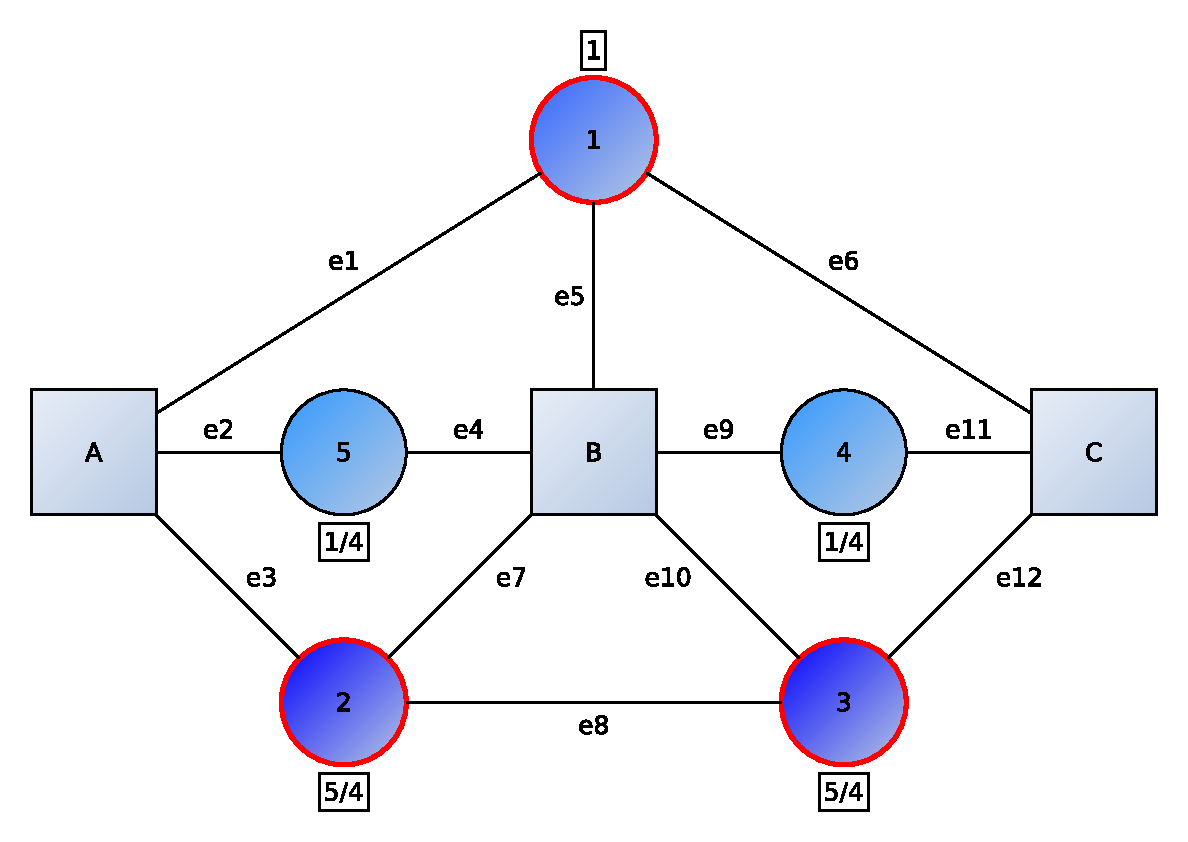
\includegraphics[scale=0.60]{./img/exemple1suite}
	\caption{Exemple (suite) $C_{I}$ ordonné}
	\label{fig:exemple1suite}
\end{figure}

\section{Implémentation, tests}

\section{Discussion}

\begin{todo} Prendre en compte :
	\begin{itemize}
		\item Nombre de chemins passant par les $c$
		\item Les poids sur les noeuds, voir les arêtes
		\item Signature des chemins ?
	\end{itemize}
	Voir du coté de \og betweenness centrality \fg, concept qui a l'air très proche.
\end{todo}
